\documentclass[11pt,a4paper]{article}
\usepackage[utf8]{inputenc}
\usepackage[T1]{fontenc}
\usepackage[margin=2.4cm]{geometry}
\usepackage{amsmath,amssymb}
\usepackage{graphicx}
\usepackage{booktabs}
\usepackage{listings}
\usepackage{xcolor}
\usepackage[colorlinks=true,linkcolor=blue!50!black,urlcolor=blue!50!black]{hyperref}

\definecolor{shade}{gray}{0.96}
\lstset{
  basicstyle=\ttfamily\footnotesize, backgroundcolor=\color{shade},
  keywordstyle=\color{blue!60!black}, commentstyle=\color{green!35!black}\itshape,
  stringstyle=\color{red!60!black}, language=Python, showstringspaces=false,
  breaklines=true, frame=leftline, framerule=1.2pt, rulecolor=\color{gray!50},
  xleftmargin=10pt, aboveskip=8pt, belowskip=8pt}

\newcommand{\why}[1]{\medskip\noindent\textbf{Why:} #1\medskip}

\title{\vspace{-1.5cm}\textbf{Two-body low-energy scattering}\\[6pt]
       \large Theory and implementation: every function, every constant, and why}
\author{Pedro Henrique Gesualdo Modesto\\
        \small São Carlos Institute of Physics --- University of São Paulo}
\date{\today}

\begin{document}
\maketitle

\begin{abstract}
\noindent
This document takes apart the two-body low-energy scattering code: every
function, every term, every parameter, and the reason behind each choice. It is
not a user manual --- it is the explanation of \emph{why}. Every numerical
constant that appears in the code has here the calculation or the measurement
that fixed it. The errors made and corrected are collected in
Sec.~\ref{sec:autopsy}, because they are the most instructive part.
\end{abstract}

\tableofcontents
\newpage

% ======================================================================
\section{What universality means here}
\label{sec:universality}

At low energy, when the de Broglie wavelength is comparable to or larger than
the range of the potential, the detailed shape of the interaction becomes
invisible. Only two numbers survive --- the \textbf{scattering length} $a$ and
the \textbf{effective range} $r_0$ --- through the effective-range expansion
\begin{equation}
  k\cot\delta_0(k) \;=\; -\frac{1}{a} \;+\; \frac{1}{2}\,r_0\,k^2 \;+\; O(k^4).
  \label{eq:ere}
\end{equation}

\textbf{This is what universality means:} the same two-parameter description
applies across physical domains that have nothing else in common. In the words
of Ref.~\cite{rbef}, \emph{``the universal behavior in the low-energy limit
enables us to draw a parallel between cold atomic gases and nuclear systems.''}

The two systems used throughout this work make the point concrete:

\begin{center}
\begin{tabular}{lrrrl}
\toprule
system & $a$ & $r_0$ & $E$ (measured) & domain \\
\midrule
$^4$He dimer & $90.4$ \AA & $8.0$ \AA & $-1.62$ mK & atomic \\
deuteron & $5.4112$ fm & $1.7436$ fm & $-2.224$ MeV & nuclear \\
\bottomrule
\end{tabular}
\end{center}

Nine orders of magnitude apart in energy, five in length, and one is held
together by the van der Waals force while the other is held together by the
strong interaction. And yet the same two numbers, fed into the same two
formulas, reproduce both binding energies.

\subsection*{Shape independence is the mechanism, not the definition}

A separate --- and often confused --- statement is that \emph{different
potentials} tuned to the same $(a, r_0)$ give the same low-energy observables.
That is not the definition of universality; it is a consequence of the
\textbf{shape-independent approximation}, Eq.~(55) of~\cite{rbef}, which says
that $\delta_0(k)$ at low energy does not depend on the shape of the potential.
As~\cite{rbef} puts it, the fact that four very different potentials can be
tuned to the same $a$ and $r_0$, \emph{``although remarkable, is directly
related to the shape-independent approximation.''}

So the roles are:

\begin{center}
\begin{tabular}{ll}
\toprule
\textbf{universality} & two parameters describe low-energy physics across domains \\
\textbf{shape independence} & why the shape of $V$ beyond those two numbers does not matter \\
\textbf{tuning} & the numerical procedure that puts a given $V$ at a chosen $(a, r_0)$ \\
\bottomrule
\end{tabular}
\end{center}

\why{Tuning is a \emph{demonstration technique}, not a physical claim. The tuned
parameters are of course different for each potential --- a Gaussian and a
Lennard-Jones that share $(a, r_0)$ have nothing numerically in common. What
they share is everything a low-energy experiment can measure.}

\subsection*{When two parameters are not enough}

The expansion~\eqref{eq:ere} is a series, and dropping $r_0$ means keeping only
its first term. Whether that is legitimate depends on how small $kR$ is.
Reference~\cite{rbef} makes exactly this point for the deuteron: the zero-range
formula \emph{``only accounts for $\approx 64\%$ of the deuteron energy''},
because \emph{``$kR \sim 0.4$ for the deuteron is larger than in the $^4$He
case.''}

\begin{center}
\begin{tabular}{lrrr}
\toprule
system & $r_0/|a|$ & zero range & finite range \\
\midrule
deuteron & $0.32$ & $-36\%$ & $-0.05\%$ \\
$^4$He dimer & $0.089$ & $-8.6\%$ & $+0.47\%$ \\
\bottomrule
\end{tabular}
\end{center}

\why{The deuteron is the textbook example of a shallow bound state, and it is
the one that needs the finite-range correction most. Being universal is not a
property a system has or lacks in the abstract; it is a statement about how
small the expansion parameter happens to be.}

% ======================================================================
\section{Conventions and units}

The $s$-wave radial Schrödinger equation, written for $u(r) = r\,\psi(r)$, is
\begin{equation}
  -\frac{\hbar^2}{2m_r}\,u''(r) + V(r)\,u(r) = E\,u(r),
\end{equation}
with $m_r = m_1m_2/(m_1+m_2)$ the reduced mass. The code sets
$\hbar = m_r = 1$ and measures lengths in fm, so
\begin{equation}
  \boxed{\;u'' = 2\,\bigl(V - E\bigr)\,u\;}
  \label{eq:radial}
\end{equation}
which is the only equation the code ever solves, at $E = 0$ and at $E < 0$ alike.

\subsection*{Back to physical units}

Comparing~\eqref{eq:radial} with the dimensional form,
\[
  \frac{2m_r}{\hbar^2}\bigl(V_{\text{phys}} - E_{\text{phys}}\bigr)
  = 2\bigl(V_{\text{code}} - E_{\text{code}}\bigr)
  \;\Longrightarrow\;
  E_{\text{phys}} = \frac{\hbar^2}{m_r}\,E_{\text{code}},
\]
and since $\hbar^2/2m_r$ is the constant usually tabulated,
\begin{equation}
  \boxed{\;E_{\text{phys}} = 2\left(\frac{\hbar^2}{2m_r}\right) E_{\text{code}}\;}
  \label{eq:conversion}
\end{equation}

\why{That factor of 2 is easy to lose. The check that would expose it is in
Sec.~\ref{sec:data}: with it wrong, the inferred constant would not come out at
$41.47$ MeV$\cdot$fm$^2$.}

% ======================================================================
\section{The one idea: do not integrate what is already known}
\label{sec:idea}

Every potential here has a range $R$. Beyond $R$ we have $V = 0$, and there
Eq.~\eqref{eq:radial} has a solution known without computing anything:
\begin{align}
  E = 0:&\quad u'' = 0 &&\Longrightarrow\quad u \text{ is a \textbf{straight line}},\\
  E < 0:&\quad u'' = -2E\,u &&\Longrightarrow\quad u \propto e^{-\kappa r},\;\;
    \kappa = \sqrt{-2E}.
\end{align}

So the code \textbf{never integrates past $R$}. It integrates from the inner
boundary out to $R$, reads the value and the slope there, and glues the analytic
form on. All three quantities come out of that gluing:

\begin{center}
\begin{tabular}{ll}
\toprule
\textbf{quantity} & \textbf{comes from} \\
\midrule
$a$   & where the asymptotic straight line crosses zero \\
$r_0$ & the integral of the difference between that line and the true solution \\
$E$   & the energy that makes the solution glue onto the exponential \\
\bottomrule
\end{tabular}
\end{center}

\why{Integrating beyond $R$ would mean computing numerically something already
known exactly, and paying for it in numerical error.}

% ======================================================================
\section{The four potentials}

The choice is not decorative: each shape stresses a different numerical
hypothesis.

\begin{center}
\begin{tabular}{llp{5.8cm}}
\toprule
\textbf{Potential} & \textbf{Form} & \textbf{What it stresses} \\
\midrule
Square well, Eq.~(70) & $-v\mu^2$ for $r<1/\mu$ & a \textbf{discontinuity} \\
Pöschl-Teller, Eq.~(116) & $-v\mu^2/\cosh^2(\mu r)$ & \textbf{smooth and solvable} in closed form \\
Gaussian, Eq.~(120) & $-v\mu^2 e^{-\mu^2r^2}$ & tail dying \textbf{faster than exponentially} \\
Lennard-Jones, Eq.~(121) & $\tfrac12(C_{12}/r^{12} - C_6/r^6)$ & \textbf{hard core} plus van der Waals tail \\
\bottomrule
\end{tabular}
\end{center}

\begin{figure}[htbp]\centering
  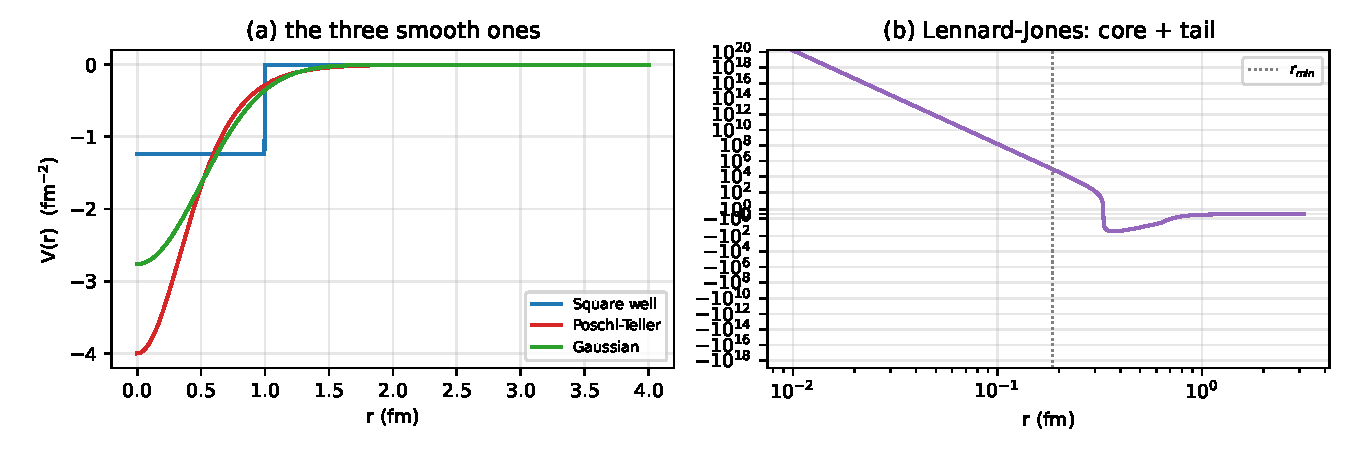
\includegraphics[width=\textwidth]{figures/potentials.pdf}
  \caption{The four potentials, all tuned to unitarity ($|a|\to\infty$). The
  Lennard-Jones needs logarithmic axes because its core reaches $10^{10}$ in
  code units; the dotted line marks \texttt{r\_min}, where integration starts.}
\end{figure}

\subsection{The range $R$, in closed form}

Each class needs to know where its potential stops acting. For the well that is
exact, $R = 1/\mu$. For the other three the potential never truly vanishes ---
a Gaussian decays forever --- so $R$ is defined as the radius where
$|V(R)| = \texttt{V\_ZERO}$, and that equation is solved \emph{on paper}:

\begin{align}
  \text{Pöschl-Teller:}&\quad \frac{v\mu^2}{\cosh^2(\mu R)} = \varepsilon
    &&\Longrightarrow\quad R = \frac{1}{\mu}\,\mathrm{arccosh}\!\sqrt{\frac{v\mu^2}{\varepsilon}}\\
  \text{Gaussian:}&\quad v\mu^2 e^{-\mu^2R^2} = \varepsilon
    &&\Longrightarrow\quad R = \frac{1}{\mu}\sqrt{\ln\frac{v\mu^2}{\varepsilon}}\\
  \text{Lennard-Jones (tail):}&\quad \tfrac12 C_6/R^6 = \varepsilon
    &&\Longrightarrow\quad R = \left(\frac{C_6}{2\varepsilon}\right)^{1/6}\\
  \text{Lennard-Jones (core):}&\quad \tfrac12 C_{12}/r_{\min}^{12} = V_{\text{core}}
    &&\Longrightarrow\quad r_{\min} = \left(\frac{C_{12}}{2V_{\text{core}}}\right)^{1/12}
\end{align}

\why{An earlier version searched for these radii numerically, sweeping a global
40\,000-point grid. Solving on paper removed that grid, removed a helper
function, and made the result exact instead of limited by the sweep resolution.}

\subsection{A factor of two in Eq.~(121)}
\label{sec:halffactor}

Equation~(121) of~\cite{rbef} reads
\[ V_{LJ}(r) = \frac{\hbar^2}{m_r}\left(\frac{C_{12}}{r^{12}} - \frac{C_6}{r^6}\right), \]
which in the units used here is $C_{12}/r^{12}-C_6/r^6$, with \textbf{no}
$\tfrac12$. Taken literally, it does not reproduce Table~4 of the same paper.
Using the published deuteron parameters $C_{12} = 0.90485319$ and
$C_6 = 6.81472$:

\begin{center}
\begin{tabular}{lrr}
\toprule
& $a$ (fm) & $r_0$ (fm) \\
\midrule
Table 4 of~\cite{rbef} & $5.4$ & $1.70$ \\
with the $\tfrac12$ & $5.405$ & $1.699$ \\
without it & $\mathbf{1.435}$ & $1.412$ \\
\bottomrule
\end{tabular}
\end{center}

Equations~(70) and (120), for the well and the Gaussian, carry the same
$\hbar^2/m_r$ prefactor and \emph{do} reproduce Table~3 exactly as printed. The
mismatch is therefore specific to Eq.~(121); the likely reading is $2m_r$ in its
denominator. The code uses the $\tfrac12$.

\why{This is the kind of detail that survives unnoticed because the result
\emph{looks} right either way --- the curves have the expected shape. Only the
numerical comparison against the published table exposes it.}

% ======================================================================
\section{Numerov: the integrator}

Numerov solves equations of the form $u'' = W(r)\,u$, which is exactly
Eq.~\eqref{eq:radial} with $W = 2(V-E)$. The recursion is
\begin{equation}
  u_{i+1} = \frac{\bigl(12 - 10 f_i\bigr)u_i - f_{i-1}u_{i-1}}{f_{i+1}},
  \qquad f_i = 1 - \frac{h^2 W_i}{12}.
  \label{eq:numerov}
\end{equation}

\subsection*{Where it comes from}

Expanding $u_{i\pm1}$ in Taylor series and adding,
\[
  u_{i+1} + u_{i-1} = 2u_i + h^2 u_i'' + \frac{h^4}{12}u_i^{(4)} + O(h^6).
\]
A second-order method simply discards the $h^4$ term. Numerov does not: since
$u'' = Wu$, we have $u^{(4)} = (Wu)''$, and that second derivative can be
approximated by the \emph{same} central difference, without evaluating anything
at new points. Substituting and regrouping gives Eq.~\eqref{eq:numerov}.

\why{This is why Numerov reaches order $h^4$ at the cost of a second-order
scheme: it never evaluates $W$ away from the grid. The price is a
\emph{three-term} recursion --- each point depends on the two before it, so an
error made at the start travels all the way out.}

\begin{lstlisting}
    f = 1.0 - h * h * W / 12.0
    for i in range(1, POINTS - 1):
        w[i + 1] = ((12.0 - 10.0 * f[i]) * w[i] - f[i - 1] * w[i - 1]) / f[i + 1]
\end{lstlisting}

% ======================================================================
\section{The logarithmic grid}
\label{sec:log}

\subsection{The problem}

Numerov requires $h\sqrt{|W|}\ll 1$ to represent the solution. Measured across
the four potentials on a uniform grid:

\begin{center}
\begin{tabular}{lrrl}
\toprule
\textbf{potential} & $h$ (fm) & $\max|W|$ & $h\sqrt{|W|}$ \\
\midrule
square well & 0.00103 & $8.3\times10^{-1}$ & 0.001 \\
Pöschl-Teller & 0.00851 & $2.1\times10^{0}$ & 0.012 \\
Gaussian & 0.00401 & $1.6\times10^{0}$ & 0.005 \\
\textbf{Lennard-Jones} & 0.00626 & $\mathbf{2.0\times10^{5}}$ & \textbf{2.78} \\
\bottomrule
\end{tabular}
\end{center}

The Lennard-Jones is squeezed from both sides: its core reaches $V=10^5$, so
$\sqrt{2V}=447$ and the characteristic length there is $0.002$ fm, while its
$1/r^6$ tail pushes $R$ out to $125$ fm. \textbf{No uniform step serves both.}

The consequence was measured, and it is a real error: the Lennard-Jones $r_0$
\emph{drifted} as the number of points doubled, instead of converging.

\begin{figure}[htbp]\centering
  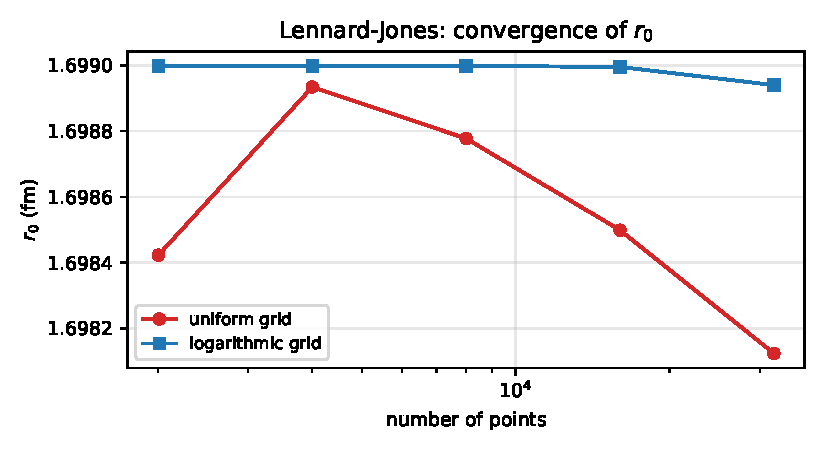
\includegraphics[width=0.72\textwidth]{figures/convergence.pdf}
  \caption{Convergence test. On a uniform grid (red) $r_0$ never settles. On a
  logarithmic grid (blue) it locks in at the fifth decimal. A result that moves
  when the grid is refined is not a result.}
  \label{fig:conv}
\end{figure}

\begin{figure}[htbp]\centering
  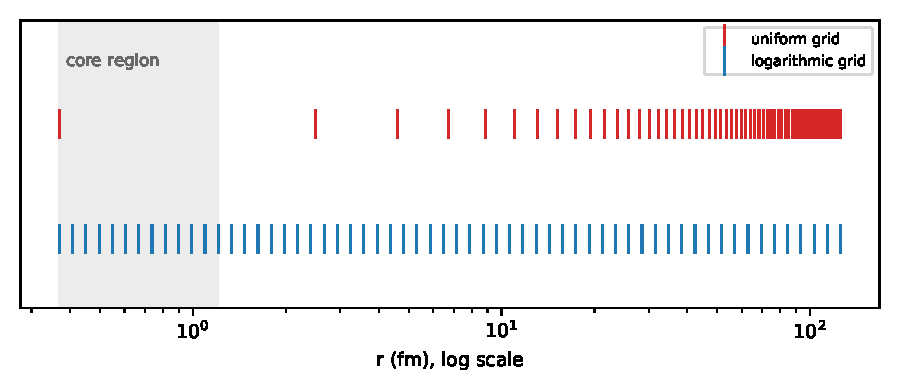
\includegraphics[width=0.8\textwidth]{figures/grid.pdf}
  \caption{Point distribution, same number of points in both cases. The uniform
  grid wastes almost everything on the tail and leaves the core with a handful
  of points; the logarithmic grid does the opposite.}
\end{figure}

\subsection{The calculation}

With $r = e^x$ and $u = e^{x/2}w(x)$, using $\dfrac{d}{dr} = e^{-x}\dfrac{d}{dx}$:
\begin{align}
  u' &= e^{-x}\frac{d}{dx}\bigl(e^{x/2}w\bigr)
      = e^{-x/2}\Bigl(\tfrac12 w + w'\Bigr),\\[4pt]
  u'' &= e^{-x}\frac{d}{dx}\Bigl[e^{-x/2}\bigl(\tfrac12 w + w'\bigr)\Bigr]
       = e^{-3x/2}\Bigl(w'' - \tfrac14 w\Bigr).
\end{align}
Substituting into Eq.~\eqref{eq:radial}, $e^{-3x/2}(w''-\tfrac14 w) = 2(V-E)e^{x/2}w$, so
\begin{equation}
  \boxed{\;w''(x) = \Bigl[\,2\bigl(V(e^x)-E\bigr)e^{2x} + \tfrac14\,\Bigr]\,w(x)\;}
  \label{eq:log}
\end{equation}

Two things matter here. First, a $\tfrac14$ \textbf{appears} that was not in the
original equation --- it comes from the substitution $u = e^{x/2}w$, not from
the physics. Second, and decisively: Eq.~\eqref{eq:log} is still of the form
$w'' = W w$, which is the \emph{only} thing Numerov requires. The recursion does
not change at all; only what goes into it does.

\why{Changing the independent variable is the standard move when a problem has
two very different scales. Here they differ by five orders of magnitude:
$0.002$ fm in the core against $125$ fm in the tail.}

\begin{lstlisting}
    r_start = pot.r_min if pot.r_min > 0.0 else pot.R * 1e-6
    x = np.linspace(math.log(r_start), math.log(pot.R), POINTS)
    h = x[1] - x[0]
    r = np.exp(x)
    W = 2.0 * (pot.V(r) - E) * r * r + 0.25
\end{lstlisting}

% ======================================================================
\section{The two starts}

Numerov needs \emph{two} initial values, and the code picks between two cases:

\begin{lstlisting}
    if pot.r_min > 0.0:
        w[1] = h * math.exp(x[0] / 2.0)      # hard core: u = 0, u' = 1 there
    else:
        w[0] = math.sqrt(r[0])               # regular origin: u ~ r
        w[1] = math.sqrt(r[1])
\end{lstlisting}

\textbf{Regular origin} (well, Pöschl-Teller, Gaussian). Near $r=0$ with finite
$V$, the regular solution behaves as $u \simeq r$. Since
$w = u\,e^{-x/2} = u/\sqrt{r}$, that gives $w \simeq \sqrt{r}$, which is exactly
what the code writes.

\textbf{Hard core} (Lennard-Jones). There $V$ blows up and $u$ is exponentially
small; we impose $u(r_{\min}) = 0$ with unit slope, and the same conversion
$w = u/\sqrt{r}$ gives $w_1 \simeq h\,e^{x_0/2}$.

\why{Getting the start wrong is not a local mistake: by the three-term
recursion, the error propagates through the whole integration. A measurement
from this work: for the Lennard-Jones, the fourth-order start correction
$u_1 = h + h^3W_0/6$ amounts to \emph{129\%} of $h$. It did not fix that
version's problem --- the cause was the grid --- but it shows the scale of what
is at stake.}

% ======================================================================
\section{The slope at the edge}

Gluing the solution onto the analytic form needs $u(R)$ and $u'(R)$. The value
comes out directly; the derivative uses a five-point one-sided difference:
\begin{equation}
  \frac{dw}{dx}\Big|_{R} \simeq
  \frac{25w_{N} - 48w_{N-1} + 36w_{N-2} - 16w_{N-3} + 3w_{N-4}}{12h}
  \;+\; O(h^4),
\end{equation}
and the conversion back to physical radius comes from the first line of the
calculation in Sec.~\ref{sec:log}:
\begin{equation}
  \frac{du}{dr}\Big|_{R} = e^{-x_N/2}\Bigl(\tfrac12 w_N + \frac{dw}{dx}\Big|_R\Bigr).
\end{equation}

\why{Two reasons for the one-sided formula instead of a central difference. It
is order $h^4$, matching the rest of the method --- a central one would be
$O(h^2)$ and would spoil the global order. And it uses \emph{interior points
only}, so it never crosses the square well's discontinuity.}

\subsection*{The discontinuity finding}

If a Numerov step straddles the well's jump, the method assumes $W$ is smooth
across the three points it uses --- and it is not. The convergence order was
measured:

\begin{center}
\begin{tabular}{rrl}
\toprule
$n$ & error in $a$ & measured order \\
\midrule
2001  & $8.9\times10^{-4}$ & --- \\
4001  & $4.5\times10^{-4}$ & 1.00 \\
8001  & $2.2\times10^{-4}$ & 1.00 \\
16001 & $1.1\times10^{-4}$ & 1.00 \\
\bottomrule
\end{tabular}
\end{center}

Order exactly 1, not 4. With the grid ending on the edge and the one-sided
derivative, the same case drops to $1.9\times10^{-10}$ --- \textbf{six orders of
magnitude}, with the same number of points.

% ======================================================================
\section{What the code measures: $a$ and $r_0$}

\subsection{The scattering length}

Beyond $R$ the solution is the straight line $u = C(1 - r/a)$. It crosses zero
at $r=a$, and knowing $u(R)$ and $u'(R)$ fixes the line:
\begin{equation}
  \boxed{\;a = R - \frac{u(R)}{u'(R)}\;}
\end{equation}

\why{This is an \emph{exact reading}, not a fit. No least squares, no
extrapolation. The only source of error is the integration out to $R$.}

The code handles $u'(R)=0$ separately: the line is horizontal, never crosses
zero, and $a = \infty$. That is exact unitarity, not a failure.

\begin{lstlisting}
    if slope == 0.0:
        a = math.inf
    else:
        a = pot.R - u[-1] / slope
\end{lstlisting}

\subsection{The normalisation, and why it is needed}

Equation~\eqref{eq:radial} is homogeneous: if $u$ is a solution, so is $Cu$. The
start chose an arbitrary normalisation, so $u$ is not yet comparable with
anything. We fix it by requiring that it meet the line at the edge:
\begin{equation}
  u \;\longleftarrow\; u\,\frac{1 - R/a}{u(R)}
  \qquad\Longrightarrow\qquad u(R) = g_0(R), \quad g_0(r) \equiv 1 - \frac{r}{a}.
\end{equation}

\why{Without this the effective-range integral would not be defined --- it
compares $u$ against $g_0$, and the comparison only makes sense once both are on
the same scale.}

\subsection{The effective range}

\begin{equation}
  r_0 = 2\int_0^\infty \Bigl[g_0(r)^2 - u(r)^2\Bigr]dr .
  \label{eq:r0}
\end{equation}

The integrand measures \emph{how far the true solution departs from the line},
which is why it is a measure of the size of the potential. Outside the range
$u = g_0$ and the integrand vanishes identically, so the integral does end at $R$.

Two details in the code:

\textbf{The factor $r$.} On the logarithmic grid $dr = r\,dx$, so the integral
becomes $\int(\dots)\,r\,dx$. That is where the \texttt{* r} in the Simpson call
comes from.

\textbf{The analytic piece.} The grid starts at $r_{\text{start}}$, not at zero.
The stretch $[0, r_{\text{start}}]$ is added by hand: there $u$ is either zero
(inside a hard core) or proportional to $r$, and in both cases its contribution
is $O(r_{\text{start}}^3)$ while the line's is $O(r_{\text{start}})$, leaving
\begin{equation}
  2\int_0^{s}g_0^2\,dr = 2\left(s - \frac{s^2}{a} + \frac{s^3}{3a^2}\right),
  \qquad s \equiv r_{\text{start}}.
\end{equation}

\why{This term used to apply only to the Lennard-Jones. Measurement showed the
square well carried a residual error of $2.4\times10^{-6}$ in $r_0$ that was
exactly this missing piece. Making the term unconditional removed an
\texttt{if} \emph{and} improved precision by three orders of magnitude --- down
to $5.6\times10^{-12}$.}

\begin{lstlisting}
    r0 = 2.0 * simpson((line ** 2 - u ** 2) * r, x=x)
    s = r_start
    r0 = r0 + 2.0 * (s - s ** 2 / a + s ** 3 / (3.0 * a ** 2))
\end{lstlisting}

% ======================================================================
\section{Counting bound states}

The code counts \emph{zeros of the zero-energy solution}. It is a striking fact
that the scattering solution, at $E=0$, knows how many bound states the
potential has.

Reference~\cite{rbef} treats this as a mandatory check rather than as a result:
\emph{``checking the number of nodes of the radial function is necessary to
guarantee that it is indeed the situation we wanted to reproduce''}, expecting a
nodeless $u(r)$ for $a<0$ and one node for $a>0$.

There is a subtlety. Beyond the edge the solution is the line $g_0 = 1 - r/a$,
which crosses zero at $r = a$. If $a > R$ that zero is physical and counts. If
$a$ is effectively infinite, the zero sits at infinity and does not --- hence
the test \texttt{R < a < 1e4}.

\begin{lstlisting}
    nodes = 0
    for i in range(1, POINTS - 1):
        if u[i] * u[i + 1] < 0.0:
            nodes = nodes + 1
    if pot.R < a < 1e4:
        nodes = nodes + 1
\end{lstlisting}

\why{The count is not optional. Two solutions can share $(a, r_0)$ and differ in
node count --- and then they are \emph{not} the same physical state. Every
tuning ends by checking it.}

\textbf{A bug that lived here:} the loop starts at \texttt{i = 1}, not
\texttt{i = 0}. Since $u_0 = 0$ by construction, including the first point
counted a spurious sign change and inflated the count by one for \emph{every}
potential.

% ======================================================================
\section{The bound state}

Beyond the edge, with $E<0$, the solution must be the decaying exponential. That
gives the matching condition
\begin{equation}
  \boxed{\;g(E) \equiv u'(R) + \kappa\,u(R) = 0,\qquad \kappa = \sqrt{-2E}\;}
\end{equation}

\why{We write the \emph{sum}, not $u'/u + \kappa$, because $u(R)$ can pass
through zero --- the deuteron has a node --- and the division would invent a
spurious pole for the root finder to chase. This cost hours: with the ratio, the
helium dimer came out completely wrong.}

\subsection*{Why there is no search}

The finite-range formula already delivers the answer to about 1\%. It is the
guess, and \texttt{brentq} merely refines it within $[1.8\,g,\;0.3\,g]$:

\begin{lstlisting}
    return brentq(gap, 1.8 * guess, 0.3 * guess, xtol=1e-15)
\end{lstlisting}

\why{An earlier version scanned 120 energies on a logarithmic grid just to find
where the function changed sign. That was waste: the approximate answer was
already in hand and was being ignored. Replacing the scan by the guess made the
calculation $3.5\times$ faster \emph{and} more accurate. There is also a
conceptual bonus: the bracket always working is itself a statement that the
effective-range expansion is good.}

% ======================================================================
\section{The inverse problem: tuning}

Given a target $(a, r_0)$, find the parameters. It is a nonlinear $2\times2$
system, and $a$ has \emph{poles}: it jumps from $+\infty$ to $-\infty$ every
time a new bound state appears.

\subsection{Two nested loops}

\begin{center}
\begin{tabular}{ll}
\toprule
\texttt{tune} & outer loop: moves the \textbf{scale} until $r_0$ matches \\
\quad\texttt{match\_a} & inner loop: moves the \textbf{strength} until $1/a$ matches \\
\quad\quad\texttt{find\_root} & widens a bracket until the sign flips, then bisects \\
\bottomrule
\end{tabular}
\end{center}

Each loop solves \emph{one} equation in \emph{one} variable. Inside the outer
loop, \texttt{r0\_error} runs the entire inner loop again for every scale it
tries --- which is why this is the slow part, about 35 of the 54 seconds.

\subsection*{The decision that makes it work: chase $1/a$}

\why{$a$ has poles; $1/a$ is smooth and crosses zero. Bisection \emph{dies} on a
pole and thrives on a zero. As a bonus, unitarity becomes $1/a = 0$ and needs no
special case at all.}

\begin{lstlisting}
    if math.isinf(a_target):
        inv_a_target = 0.0
    else:
        inv_a_target = 1.0 / a_target
\end{lstlisting}

\subsection*{Why not a 2D Newton}

The level sets of $1/a$ and $r_0$ in the (strength, scale) plane are
\emph{nearly parallel} over much of the domain. A Newton solver on both
equations at once would meet an ill-conditioned Jacobian exactly there, and take
large steps in the wrong direction. Nested bisection cannot diverge once the
sign is bracketed --- slower per iteration and far more reliable for code
someone else will run.

\subsection*{The six return values}

\texttt{tune} returns \texttt{(strength, scale, a, r0, nodes, ok)}. The last is a
flag: false if $r_0$ failed to converge \emph{or} if the node count missed its
target. Without it, a tuning that landed on the wrong state would pass unnoticed.

\why{What comes out of \texttt{tune} is a different pair of numbers for every
potential --- there is no shared parameter. What is shared is the pair
$(a, r_0)$, and with it everything a low-energy measurement can see. That is the
point of Sec.~\ref{sec:universality}.}

% ======================================================================
\section{Every constant, one by one}

No number in the code is a guess. This table is the justification for each.

\begin{center}
\begin{tabular}{lll p{6.3cm}}
\toprule
\textbf{constant} & \textbf{value} & \textbf{where} & \textbf{justification} \\
\midrule
\texttt{V\_ZERO} & $10^{-12}$ & defines $R$ &
  Below this the potential is treated as gone. Measured: cutting at $10^{-8}$
  truncates the Lennard-Jones tail and misses $r_0$ by $0.16\%$; $10^{-12}$
  closes to $0.004\%$. \\
\addlinespace
\texttt{V\_CORE} & $10^{5}$ & LJ start &
  Where integration begins inside the core. Ref.~\cite{rbef} prescribes
  $V(r_{\min}) \sim 10^{10}$; we measured that $10^{3}$ breaks the physics
  ($r_0$ off by $0.2\%$) while anything from $10^{4}$ up changes nothing.
  Starting deeper only costs stiffness. \\
\addlinespace
\texttt{POINTS} & 8001 & grid size &
  Total error is truncation (falls with $n$) plus roundoff (grows with $n$);
  8001 sits at the minimum. The three smooth potentials are at $10^{-11}$ and
  do not care. The Lennard-Jones sets the value: past $\sim$8000 its $r_0$
  \emph{degrades} again --- $3\times10^{-5}$ at 32001, $3\times10^{-4}$ at
  64001. \\
\addlinespace
\texttt{r\_start} & $R\times10^{-6}$ & regular origin &
  Where the logarithmic grid begins when there is no core. It cannot be $0$
  because $\ln 0$ does not exist. The stretch below it enters analytically. \\
\addlinespace
$[1.8g,\;0.3g]$ & --- & \texttt{brentq} &
  Bracket around the finite-range guess. It works on both systems tested; that
  it works at all is a statement about the quality of the expansion. \\
\addlinespace
$1.3$ & --- & \texttt{find\_root} &
  Bracket widening factor, up to 40 attempts. If no sign change is found it
  raises rather than returning garbage. \\
\addlinespace
$10^{-7}$, $10^{-6}$ & --- & tolerances &
  Convergence of $r_0$ in \texttt{tune} and in the tests. Measured: the tuning
  hits its target to $10^{-10}$, comfortably inside them. \\
\bottomrule
\end{tabular}
\end{center}

% ======================================================================
\section{The tabulated data}
\label{sec:data}

Five dictionaries, all traceable:

\begin{center}
\begin{tabular}{lp{10cm}}
\toprule
\texttt{TARGETS} & Table 2 of~\cite{rbef}: the three targets. The bound-state count is \emph{not} a column of that table; it comes from the text of Sec.~4.5. \\
\texttt{PUBLISHED} & Tables 3 and 4: the published parameters. Used as the initial guess \emph{and} as the validation target. \\
\texttt{SYSTEMS} & Table 1: two real systems, with measured energies. \\
\texttt{GUESS} & The deuteron solution, used as a starting point for other systems. \\
\texttt{SOURCES} & The three references with DOI, plus the \texttt{D1} divergence. \\
\bottomrule
\end{tabular}
\end{center}

\subsection{Scale invariance in \texttt{GUESS}}

The problem is scale invariant: multiplying all lengths by $L$ takes
$(a, r_0)\to(La, Lr_0)$. So attacking another system only needs the guess
rescaled:
\begin{equation}
  \mu \;\to\; \frac{\mu}{L}, \qquad C_{12} \;\to\; C_{12}\,L^6 .
\end{equation}
The $L^6$ is because $C_{12}$ multiplies $r^{-12}$.

\subsection{The constant that is tabulated nowhere}

$\hbar^2/2m_r$ appears in no table. We obtain it by inverting the zero-range
formula on the published pair $(a, E_{zr})$:
\begin{equation}
  E_{zr} = -\frac{\hbar^2/2m_r}{a^2}
  \quad\Longrightarrow\quad
  \frac{\hbar^2}{2m_r} = -E_{zr}\,a^2 .
\end{equation}

\begin{center}
\begin{tabular}{lrrl}
\toprule
system & inferred & literature & deviation \\
\midrule
deuteron & $41.462$ MeV$\cdot$fm$^2$ & $41.47$ & $0.02\%$ \\
$^4$He dimer & $12.095$ K$\cdot$\AA$^2$ & $12.12$ & $0.21\%$ \\
\bottomrule
\end{tabular}
\end{center}

\why{This is a \textbf{test}, not a convenience. Recovering both known constants
proves Table~1 is internally consistent --- and, incidentally, that the factor
of 2 in Eq.~\eqref{eq:conversion} is right.}

\subsection*{The three tunings that do not match, and why}

Nine of the twelve tunings land within $0.2\%$ of the published parameters.
Three do not, and they do not fail for the same reason.

\paragraph{Two of them are the \texttt{D1} divergence.}
(nn, Lennard-Jones) at $2.68\%$ and (deuteron, Pöschl-Teller) at $2.65\%$. The
cause is \emph{not} numerical: refining the grid moves the deviation from
$2.70\%$ to $2.69\%$. Table~3 of~\cite{rbef} reports $r_0 = 1.73$ for the mPT
deuteron row and Table~4 reports $r_0 = 2.71$ for the Lennard-Jones nn row,
while Table~2 of the same paper lists the targets as $1.70$ and $2.70$.
Feeding the published parameters back through the solver confirms it: they
produce $r_0 = 1.7300$ and $2.7080$, not the targets. We tune to the target and
land elsewhere --- correctly.

\paragraph{The third is a flat direction, not a disagreement.}
(deuteron, Lennard-Jones) sits $1.13\%$ away, but here the published parameters
\emph{do} reproduce the target: they give $r_0 = 1.6990$ against $1.7000$, an
error of $0.06\%$. Both parameter pairs are therefore valid. What happens is
that the two Lennard-Jones coefficients are strongly correlated. Starting from
the published pair and moving to ours:

\begin{center}
\begin{tabular}{lr}
\toprule
change & effect on $r_0$ \\
\midrule
$C_{12}$ alone, $+0.47\%$ & $-1.09\%$ \\
$C_6$ alone, $+1.12\%$ & $+1.18\%$ \\
both together & $\mathbf{+0.05\%}$ \\
\bottomrule
\end{tabular}
\end{center}

\noindent
Each coefficient on its own moves $r_0$ by about $1\%$; together they cancel.
The inversion $(a, r_0) \to (C_{12}, C_6)$ has a nearly flat direction, so the
observable is pinned down far more tightly than the parameters that produce it.
This is worth stating plainly because the naive reading --- ``the parameters
disagree by $1\%$, so something is wrong'' --- is exactly backwards. Note also
that Lennard-Jones is the \emph{most} sensitive of the four potentials
($\mathrm{d}\ln r_0 / \mathrm{d}\ln C_{12} = 2.28$, against $0.42$ for the well),
so the flatness comes from the correlation between the two coefficients, not
from any insensitivity of the potential.

\begin{quote}
\textbf{General rule:} a discrepancy that survives refinement is never numerical.
\end{quote}

% ======================================================================
\section{The checks}

\texttt{test\_lab.py} runs eight checks, and every one compares against
something the code did \textbf{not} compute:

\begin{center}
\begin{tabular}{lp{8cm}}
\toprule
\textbf{check} & \textbf{external anchor} \\
\midrule
$a$ of the well & Eq.~(80) of~\cite{rbef}, closed form \\
$r_0$ of the well & Eq.~(92) of~\cite{rbef}, closed form \\
$r_0/R = 1$ at the poles & exact prediction, caption of Fig.~6 of~\cite{rbef} \\
bound state & analytic condition $k\cot(kR) = -\kappa$ \\
node counts & Table 2, all 12 cases \\
tuning & Tables 3 and 4, all 12 cases \\
inferred constants & $41.47$ and $12.12$ from the literature \\
grid convergence & halving the points may change nothing \\
\bottomrule
\end{tabular}
\end{center}

\why{No check says ``same as last time''. Such a check would only prove the code
is consistent with its own mistakes.}

The last one is what \emph{found} the uniform-grid bug. It halves the points
rather than doubling them, deliberately: since the total error has a minimum,
the useful question is ``have we converged coming from below?'' and not ``what
happens deep in the roundoff regime?''.

% ======================================================================
\section{Autopsy: the errors made}
\label{sec:autopsy}

This section exists because the cause of an error is usually worth more than the
result.

\subsection*{1. Numerov dropping from order 4 to order 1}
\textbf{Symptom:} the square well converged far too slowly.
\textbf{Cause:} a step straddled the discontinuity; Numerov assumes $W$ is
smooth across the three points it uses. \textbf{Fix:} the grid ends exactly on
the edge and the derivative uses interior points only. \textbf{Gain:} six orders
of magnitude.

\subsection*{2. The Lennard-Jones $r_0$ drifting}
\textbf{Symptom:} $1.74257 \to 1.74215 \to 1.74165$ as the points doubled.
\textbf{Diagnosis:} two wrong hypotheses were discarded before the right one ---
it was not the tail (truncating at 30 fm kept the drift) and not the start
(a fourth-order correction changed nothing). It was $h\sqrt{|W|} = 2.78$ in the
core. \textbf{Fix:} logarithmic grid. \textbf{Confirmation:} the new value
agrees with an independent method to seven digits.

\subsection*{3. Matching inside the well}
\textbf{Symptom:} the well's energy came out $0.44\%$ wrong.
\textbf{Cause:} the match used the \emph{last} point where the potential still
acted --- which, in a well, is inside, where $V\neq0$. \textbf{Fix:} match
outside.

\subsection*{4. The spurious node at the origin}
\textbf{Symptom:} every potential reported one extra bound state.
\textbf{Cause:} $u_0 = 0$ by construction counted as a sign change.
\textbf{Fix:} start the loop at \texttt{i = 1}.

\subsection*{5. The inner term that only applied to the Lennard-Jones}
\textbf{Symptom:} residual error of $2.4\times10^{-6}$ in the well's $r_0$.
\textbf{Cause:} the logarithmic grid does not cover $[0, r_{\text{start}}]$, and
the analytic term sat inside an \texttt{if}. \textbf{Fix:} make it
unconditional --- one \texttt{if} fewer and three orders of magnitude better.

\subsection*{6. Citations taken on trust}
\textbf{Symptom:} three potentials were attributed to the wrong equation numbers
(74 instead of 70, 118 instead of 120, 120 instead of 121), and the node
counting was attributed to a theorem that the paper never mentions.
\textbf{Cause:} the citations were written from memory rather than checked
against the source. \textbf{Fix:} a full pass with the paper open, which also
turned up the factor of two in Sec.~\ref{sec:halffactor}.
\textbf{Lesson:} a plausible citation and a verified citation look identical on
the page.

% ======================================================================
\section{Results}

\begin{figure}[htbp]\centering
  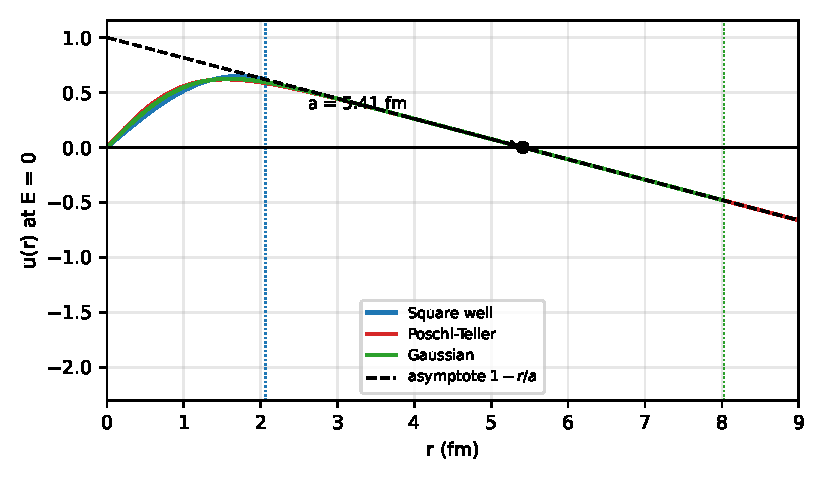
\includegraphics[width=0.72\textwidth]{figures/wavefunctions.pdf}
  \caption{Three potentials tuned to the same $(a, r_0)$ of the deuteron: the
  wavefunctions are \emph{identical outside} the range and \emph{completely
  different inside}. Dotted lines mark where each potential ends. Everything a
  low-energy experiment can see lives outside.}
\end{figure}

\begin{figure}[htbp]\centering
  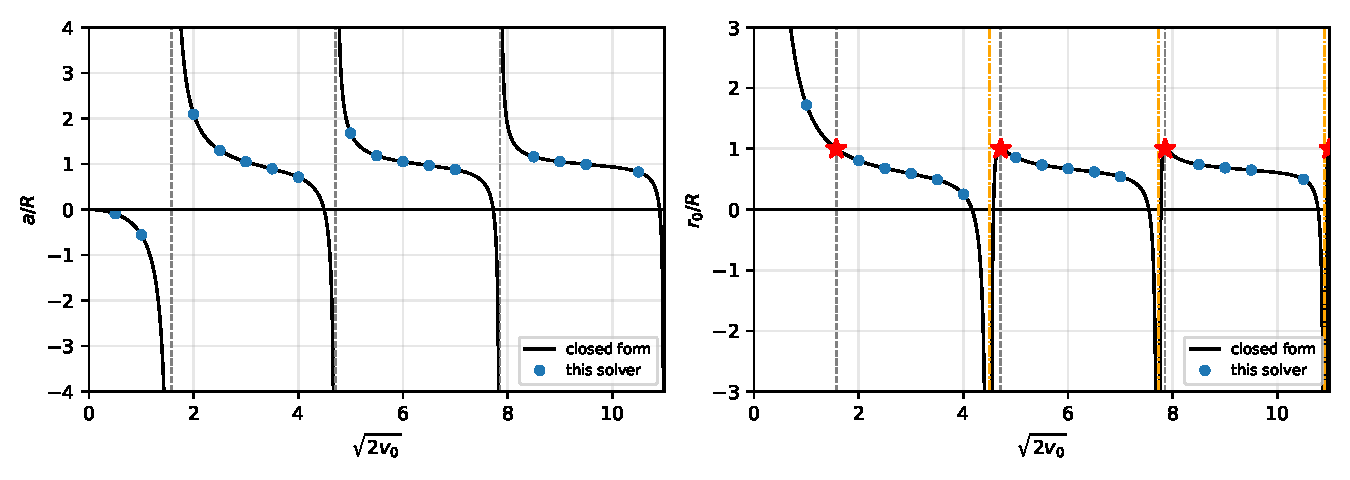
\includegraphics[width=\textwidth]{figures/article56.pdf}
  \caption{Reproduction of Figs.~5 and 6 of~\cite{rbef}. Left: $a/R$ diverges at
  $\sqrt{2v_0} = \pi/2 + n\pi$, where a new bound state appears. Right: at each
  of those points $r_0/R = 1$ \emph{exactly} (red stars), as stated in the
  caption of Fig.~6 of~\cite{rbef}. Orange lines mark the \emph{other} family of
  singularities, the roots of $\tan x = x$, where $a=0$ and it is $r_0$ that
  diverges.}
\end{figure}

\subsection{Binding energies}

\begin{center}
\begin{tabular}{lrr rr}
\toprule
& \multicolumn{2}{c}{\textbf{deuteron} ($r_0/|a| = 0.32$)}
& \multicolumn{2}{c}{\textbf{$^4$He dimer} ($r_0/|a| = 0.089$)} \\
\cmidrule(lr){2-3}\cmidrule(lr){4-5}
method & $E$ (MeV) & deviation & $E$ (K) & deviation \\
\midrule
experiment        & $-2.224$ & --- & $-1.620\times10^{-3}$ & --- \\
zero range        & $-1.416$ & $-36.3\%$ & $-1.480\times10^{-3}$ & $-8.6\%$ \\
finite range      & $-2.223$ & $-0.05\%$ & $-1.628\times10^{-3}$ & $+0.47\%$ \\
\midrule
square well       & $-2.204$ & $-0.91\%$ & $-1.627\times10^{-3}$ & $+0.46\%$ \\
Pöschl-Teller     & $-2.227$ & $+0.11\%$ & $-1.628\times10^{-3}$ & $+0.47\%$ \\
Gaussian          & $-2.214$ & $-0.47\%$ & $-1.627\times10^{-3}$ & $+0.46\%$ \\
Lennard-Jones     & $-2.203$ & $-0.92\%$ & --- & --- \\
\bottomrule
\end{tabular}
\end{center}

Two systems separated by nine orders of magnitude in energy, described by the
same two numbers and the same two formulas. That is the universality of
Sec.~\ref{sec:universality}, measured.

The residual spread of about $1\%$ \emph{among} the potentials is the shape
dependence --- the $O(k^4)$ terms, the only thing still distinguishing a square
well from a Lennard-Jones once $a$ and $r_0$ are fixed.

\subsection{Accuracy achieved}

\begin{center}
\begin{tabular}{lr}
\toprule
check & error \\
\midrule
$a$ of the well against Eq.~(80) & $1.9\times10^{-10}$ \\
$r_0$ of the well against Eq.~(92) & $5.6\times10^{-12}$ \\
bound state against $k\cot(kR)=-\kappa$ & $3.4\times10^{-10}$ \\
$r_0/R$ at the four poles & $1.0000000000$ \\
solver against closed forms (16 points) & $8.4\times10^{-9}$ \\
tuning hitting its target & $10^{-10}$ \\
\bottomrule
\end{tabular}
\end{center}

% ======================================================================
\section{What is missing}

\textbf{No error bars.} No number here carries an estimated discretisation
uncertainty.

\textbf{No Aziz HFD-B potential.} Reference~\cite{rbef} also benchmarks against
the realistic \emph{ab initio} He--He potential. This work uses four model
potentials only.

\textbf{No variable phase method.} An independent second route to $a$, which
would give a cross-check on the least reliable number here.

\textbf{No finite-$k$ phase shift.} Everything is done at $E=0$, with $r_0$ from
the integral. Computing $\delta_0(k)$ and fitting Eq.~\eqref{eq:ere} would be an
independent validation --- and is the test that would settle the Lennard-Jones
$r_0$, reliable only to $\sim10^{-6}$ and limited by roundoff.

\textbf{$s$-wave only,} valid while $kR \ll 1$.

% ======================================================================
\begin{thebibliography}{9}
\bibitem{rbef}
  M.~Macêdo-Lima and L.~Madeira,
  \emph{Scattering length and effective range of microscopic two-body potentials},
  Rev.\ Bras.\ Ensino Fís.\ \textbf{45}, e20230079 (2023).
  \href{https://doi.org/10.1590/1806-9126-RBEF-2023-0079}{doi:10.1590/1806-9126-RBEF-2023-0079}

\bibitem{hack}
  R.~W.~Hackenburg,
  \emph{Low-energy neutron-proton effective range parameters},
  Phys.\ Rev.\ C \textbf{73}, 044002 (2006).
  \href{https://doi.org/10.1103/PhysRevC.73.044002}{doi:10.1103/PhysRevC.73.044002}

\bibitem{cencek}
  W.~Cencek \emph{et al.},
  \emph{Effects of adiabatic, relativistic, and QED corrections on the pair
  potential of helium},
  J.\ Chem.\ Phys.\ \textbf{136}, 224303 (2012).
  \href{https://doi.org/10.1063/1.4712218}{doi:10.1063/1.4712218}
\end{thebibliography}


% ======================================================================
\appendix
\section{The three functions in full}

The body of the central functions, so that no line is left unexplained. The
numbered comments refer to the notes below each block.

\subsection{\texttt{numerov} --- the integrator}

\begin{lstlisting}
def numerov(pot, E):
    r_start = pot.r_min if pot.r_min > 0.0 else pot.R * 1e-6          # (1)

    x = np.linspace(math.log(r_start), math.log(pot.R), POINTS)       # (2)
    h = x[1] - x[0]
    r = np.exp(x)
    W = 2.0 * (pot.V(r) - E) * r * r + 0.25                           # (3)
    f = 1.0 - h * h * W / 12.0                                        # (4)

    w = np.zeros(POINTS)
    if pot.r_min > 0.0:
        w[1] = h * math.exp(x[0] / 2.0)                               # (5)
    else:
        w[0] = math.sqrt(r[0])                                        # (6)
        w[1] = math.sqrt(r[1])
    for i in range(1, POINTS - 1):
        w[i + 1] = ((12.0 - 10.0*f[i]) * w[i] - f[i-1]*w[i-1]) / f[i+1]   # (7)

    u = np.exp(x / 2.0) * w                                           # (8)

    dwdx = (25.0*w[-1] - 48.0*w[-2] + 36.0*w[-3]
            - 16.0*w[-4] + 3.0*w[-5]) / (12.0 * h)                    # (9)
    slope = math.exp(-x[-1] / 2.0) * (0.5 * w[-1] + dwdx)             # (10)

    return r, u, x, h, slope, r_start
\end{lstlisting}

\begin{enumerate}\setlength\itemsep{1pt}
\item Where to start: outside the core if there is one, otherwise near the
      origin, because $\ln 0$ does not exist. The skipped stretch enters
      analytically.
\item The grid is uniform in $x = \ln r$ and ends \emph{exactly} at $\ln R$.
\item The effective potential of Eq.~\eqref{eq:log}. The $r^2$ comes from
      $e^{2x}$; the $0.25$ is the $\tfrac14$ the substitution generated.
\item Numerov's $f$. Note it is a \emph{vector}, computed once for the whole
      grid before the loop.
\item Hard-core start: $u=0$, $u'=1$, converted through $w = u/\sqrt{r}$.
\item Regular start: $u\simeq r$, hence $w\simeq\sqrt{r}$. Two points are needed
      because the recursion has three terms.
\item The recursion. It is the only line that actually integrates the equation.
\item Back from $w$ to $u$. From here on everything is in physical units.
\item Five-point one-sided derivative, order $h^4$, interior points only.
\item Conversion of the derivative to radius: $du/dr = e^{-x/2}(w/2 + dw/dx)$.
\end{enumerate}

\subsection{\texttt{scattering} --- the three readings}

\begin{lstlisting}
def scattering(pot):
    r, u, x, h, slope, r_start = numerov(pot, 0.0)                    # (1)

    if slope == 0.0:
        a = math.inf                                                  # (2)
    else:
        a = pot.R - u[-1] / slope

    u = u * (1.0 - pot.R / a) / u[-1]                                 # (3)
    line = 1.0 - r / a

    r0 = 2.0 * simpson((line ** 2 - u ** 2) * r, x=x)                 # (4)
    s = r_start
    r0 = r0 + 2.0 * (s - s**2 / a + s**3 / (3.0 * a**2))              # (5)

    nodes = 0
    for i in range(1, POINTS - 1):                                    # (6)
        if u[i] * u[i + 1] < 0.0:
            nodes = nodes + 1
    if pot.R < a < 1e4:
        nodes = nodes + 1                                             # (7)

    return a, r0, nodes
\end{lstlisting}

\begin{enumerate}\setlength\itemsep{1pt}
\item Zero energy: the only case in which the exterior solution is a straight line.
\item A horizontal line means exact unitarity, and $a=\infty$ is the right
      answer --- not an error to be avoided.
\item The normalisation. Without it the following integral would not be defined,
      because the equation is homogeneous.
\item The integral of Eq.~\eqref{eq:r0}. The \texttt{* r} is the Jacobian
      $dr = r\,dx$.
\item The stretch $[0, r_{\text{start}}]$, done on paper.
\item The loop starts at 1: including $u_0=0$ would count a spurious node.
\item The exterior node at $r=a$, which exists only if $a$ is finite and larger
      than $R$.
\end{enumerate}

\subsection{\texttt{tune} --- the inverse problem}

\begin{lstlisting}
def tune(name, a_target, r0_target, strength, scale, nodes_target=None):
    if math.isinf(a_target):
        inv_a_target = 0.0                                            # (1)
    else:
        inv_a_target = 1.0 / a_target

    for step in range(25):                                            # (2)
        strength = match_a(name, scale, strength, inv_a_target)       # (3)
        a, r0, nodes = scattering(POTENTIALS[name](strength, scale))
        if abs(r0 - r0_target) < 1e-7:
            break

        def r0_error(trial_scale):                                    # (4)
            s = match_a(name, trial_scale, strength, inv_a_target)
            a2, r02, n2 = scattering(POTENTIALS[name](s, trial_scale))
            return r02 - r0_target

        scale = find_root(r0_error, scale)

    strength = match_a(name, scale, strength, inv_a_target)           # (5)
    a, r0, nodes = scattering(POTENTIALS[name](strength, scale))

    ok = abs(r0 - r0_target) < 1e-6
    if nodes_target is not None and nodes != nodes_target:
        ok = False                                                    # (6)

    return strength, scale, a, r0, nodes, ok
\end{lstlisting}

\begin{enumerate}\setlength\itemsep{1pt}
\item Unitarity with no special case: $a=\infty$ is simply $1/a=0$.
\item Twenty-five attempts at most. Leaving early means it converged.
\item Inner loop: fixes the strength so that $1/a$ matches, scale held.
\item This nested function is the cost of the algorithm: for every scale it
      tries, it runs the \emph{entire} inner loop again.
\item One last adjustment of the strength, because the scale moved last.
\item The \texttt{ok} flag. Without it, a tuning that landed on the wrong state
      would pass unnoticed.
\end{enumerate}

\section{The data, with values}

\subsection*{\texttt{TARGETS} --- Table 2 of~\cite{rbef}}
\begin{center}
\begin{tabular}{lrrc}
\toprule
case & $a$ (fm) & $r_0$ (fm) & bound states \\
\midrule
\texttt{nn} (neutron-neutron) & $-18.5$ & $2.7$ & 0 \\
\texttt{unitarity} & $\pm\infty$ & $1.0$ & 0 \\
\texttt{deuteron} & $5.4$ & $1.7$ & 1 \\
\bottomrule
\end{tabular}
\end{center}
\noindent
The bound-state column is not printed in Table~2; it comes from the text of
Sec.~4.5 of~\cite{rbef}, which asks for a nodeless $u(r)$ when $a<0$ and one
node when $a>0$.

\subsection*{\texttt{PUBLISHED} --- Tables 3 and 4, against what the tuning returns}
\begin{center}
\footnotesize
\begin{tabular}{llrrrrr}
\toprule
case & potential & $p_1$ obtained & $p_1$ published & $p_2$ obtained & $p_2$ published & deviation \\
\midrule
nn & well          & 1.109228 & 1.1096 & 0.391087 & 0.3918 & 0.18\% \\
nn & Pöschl-Teller & 0.907086 & 0.9071 & 0.799622 & 0.7991 & 0.07\% \\
nn & Gaussian      & 1.211903 & 1.2121 & 0.567906 & 0.5672 & 0.12\% \\
nn & Lennard-Jones & 9.760657 & 9.8667 & 3.005560 & 3.0884 & \textbf{2.68\%} \\
\addlinespace
unit. & well          & 1.233701 & 1.2337 & 1.000000 & 1.0000 & 0.00\% \\
unit. & Pöschl-Teller & 1.000000 & 1.0000 & 2.000000 & 2.0000 & 0.00\% \\
unit. & Gaussian      & 1.342002 & 1.3420 & 1.435224 & 1.4349 & 0.02\% \\
unit. & Lennard-Jones & 0.264625 & 0.2646 & 0.000341 & 0.00034 & 0.00\% \\
\addlinespace
deut. & well          & 1.758644 & 1.7575 & 0.499215 & 0.5000 & 0.16\% \\
deut. & Pöschl-Teller & 1.423895 & 1.4388 & 0.886001 & 0.8631 & \textbf{2.65\%} \\
deut. & Gaussian      & 1.910904 & 1.9102 & 0.674817 & 0.6754 & 0.09\% \\
deut. & Lennard-Jones & 6.846862 & 6.8147 & 0.915045 & 0.9049 & 1.13\% \\
\bottomrule
\end{tabular}
\end{center}
\noindent
The two rows in bold are the \texttt{D1} divergence: the published parameters
achieve $r_0 = 2.71$ and $1.73$, while Table~2 of the same paper asks for $2.70$
and $1.70$. Refining the grid does not move these deviations. The third row
above $0.2\%$, (deut., Lennard-Jones) at $1.13\%$, is not of that kind: there
the published parameters do reach the target, and the gap is the flat direction
in $(C_{12}, C_6)$ discussed above.

\subsection*{\texttt{SYSTEMS} --- Table 1, the two real systems}
\begin{center}
\begin{tabular}{lrrrr}
\toprule
system & $a$ & $r_0$ & measured $E$ & inferred $\hbar^2/2m_r$ \\
\midrule
deuteron & $5.4112$ fm & $1.7436$ fm & $-2.224$ MeV & $41.462$ MeV$\cdot$fm$^2$ \\
$^4$He dimer & $90.4$ \AA & $8.0$ \AA & $-1.62$ mK & $12.095$ K$\cdot$\AA$^2$ \\
\bottomrule
\end{tabular}
\end{center}

\end{document}
